\documentclass[10pt,twocolumn,letterpaper]{article}

% ─────────────────────────────────────────────────────────────────────────────
% Packages
% ─────────────────────────────────────────────────────────────────────────────
\usepackage[margin=0.75in]{geometry}
\usepackage{graphicx}
\usepackage{booktabs}
\usepackage{microtype}
\usepackage{times}
\usepackage{hyperref}
\usepackage{xcolor}
\usepackage{listings}
\usepackage{algorithm}
\usepackage{algpseudocode}
\usepackage{float}
\usepackage{caption}
\usepackage{subcaption}
\usepackage{multirow}
\usepackage{array}
\usepackage{amsmath}
\usepackage{amssymb}
\usepackage{stfloats}

\hypersetup{colorlinks=true, linkcolor=blue, urlcolor=blue, citecolor=blue}

% Code styling
\lstset{
  basicstyle=\small\ttfamily,
  keywordstyle=\color{blue},
  commentstyle=\color{gray},
  stringstyle=\color{red},
  breaklines=true,
  numbers=left,
  numberstyle=\tiny,
  stepnumber=1,
  xleftmargin=2em,
  frame=single,
  language=C++
}

% Algorithm styling
\algrenewcommand\algorithmicif{\textbf{if}}
\algrenewcommand\algorithmicthen{\textbf{then}}
\algrenewcommand\algorithmicelse{\textbf{else}}
\algrenewcommand\algorithmicend{\textbf{end}}
\algrenewcommand\algorithmicfor{\textbf{for}}
\algrenewcommand\algorithmicdo{\textbf{do}}

\newcommand{\srrip}{\textsc{SRRIP}}
\newcommand{\ipv}{\textsc{IPV}}
\newcommand{\lru}{\textsc{LRU}}
\newcommand{\lfu}{\textsc{LFU}}
\newcommand{\doa}{\textsc{DoA}}
\newcommand{\bhist}{\textsc{bHIST}}
\newcommand{\phist}{\textsc{pHIST}}
\newcommand{\pfq}{\textsc{PFQ}}
\newcommand{\stlb}{\textsc{STLB}}
\newcommand{\llc}{\textsc{LLC}}
\newcommand{\rrpv}{\textsc{RRPV}}

\title{Liveness-Guided Replacement Policies for Cache Hierarchies}
\author{Oskar Tegby$^*$ and Alberto Ros}
\date{\today}

\begin{document}

\maketitle

% Adjust float handling for two-column layout
\setcounter{topnumber}{4}
\setcounter{bottomnumber}{2}
\setcounter{totalnumber}{6}
\renewcommand{\topfraction}{0.95}
\renewcommand{\bottomfraction}{0.80}
\renewcommand{\textfraction}{0.05}
\renewcommand{\floatpagefraction}{0.85}

% ─────────────────────────────────────────────────────────────────────────────
\begin{abstract}
Modern replacement policies in caches struggle to distinguish between blocks with
short remaining lifetimes (dead-on-arrival) and those with longer lifetimes.
This paper proposes augmenting Static Re-Reference Interval Prediction (\srrip)
and Insertion Policy Version (\ipv) replacement policies with liveness information
tracked via per-PC history tables. By querying dead-on-arrival statistics at
block insertion and hit time, we can make more informed replacement decisions.

We evaluate our approach at two cache levels: first the last-level cache (\llc),
where \srrip-Live achieves 4-5\% speedup on Qualcomm and 2-3\% on Google; then
the second-level TLB (\stlb), where we extend the approach with learned promotion
vectors. Applied to both cache levels simultaneously (\ipv-Live\_both), the
complementary per-page and per-block signals yield \textbf{8\% speedup on
Qualcomm and 4-5\% on Google} server workloads, demonstrating that liveness
guidance is effective across the cache hierarchy.
\end{abstract}

% ─────────────────────────────────────────────────────────────────────────────
\section{Introduction}
% ─────────────────────────────────────────────────────────────────────────────

Replacement policies in modern caches must make eviction decisions with incomplete
information about future block reuse. Traditional policies like \lru operate on
temporal locality alone, but temporal locality is not uniform across all program
counters. Some PCs repeatedly generate dead-on-arrival (blocks evicted without
further access), while others rarely do.

The key insight is that the \emph{program counter} of the instruction that
generated a cache block is a strong predictor of that block's lifetime within
the cache. By maintaining per-PC history of which blocks died on arrival, we can
apply more sophisticated insertion and promotion strategies to the standard
\srrip and \ipv policies.

This paper makes the following contributions:

\begin{enumerate}
  \item We propose PC-indexed liveness-guided variants of \srrip and \ipv that
    integrate dead-on-arrival information into replacement decisions.

  \item We introduce a PC-partitioned history table (\bhist) architecture that
    efficiently tracks liveness information per (PC, address) pair, avoiding the
    memory overhead of separate per-PC tables.

  \item We demonstrate that liveness-guided \ipv-Live replacement with 3-way
    liveness classification and learned promotion vectors achieves 8\% geomean
    speedup on Qualcomm and 4-5\% on Google when applied to both \llc and
    \stlb simultaneously, compared to 4-5\% and 2-3\% for LLC-only configurations.

  \item We show that the same approach applies to the second-level TLB (\stlb),
    where combined page-level and block-level liveness guidance provides
    additive performance improvements.
\end{enumerate}

% ─────────────────────────────────────────────────────────────────────────────
\section{Background and Motivation}
% ─────────────────────────────────────────────────────────────────────────────

\subsection{Cache Replacement and Dead-on-Arrival}

A block is considered \emph{dead-on-arrival} (\doa) if it is evicted from the
cache without ever being accessed after insertion. For a cache with size $C$ and
block size $B$, the number of blocks in the cache at any time is $C/B$. In
practice, many modern workloads exhibit high \doa rates, ranging from 10\% to
over 50\%, depending on the program and cache size.

Traditional replacement policies like \lru and \lfu treat all blocks identically
at insertion time. They do not adapt based on which instruction (\doa) is more
likely to generate short-lived accesses. This is a key missed opportunity.

\subsection{The Role of the Program Counter}

The program counter at the time of load execution is strongly correlated with
cache block lifetime. For instance:
\begin{itemize}
  \item Streaming prefetch loops often load data that is consumed once and never
    reused, leading to high \doa rates.
  \item Reuse loops that repeatedly access the same set of addresses show low
    \doa rates.
  \item Pointer-chasing traversals show intermediate \doa rates that depend on
    pointer density and working set size.
\end{itemize}

By tracking per-PC \doa statistics, we can guide the insertion and promotion
strategy for individual cache blocks.

\subsection{History Tables and Liveness Classification}

A history table is a small hardware structure that records per-PC statistics
of cache block lifetimes. In this work, we focus on tracking a single counter:
the number of times a block from PC $p$ was evicted without access (\doa count).

We classify blocks into two liveness categories:
\begin{itemize}
  \item \textbf{Dead-on-Arrival (DoA)}: When the \doa count for a (PC, address)
    pair exceeds a threshold $\theta$, we classify the block as \doa.
  \item \textbf{Mostly-Alive}: All other blocks are considered mostly-alive.
\end{itemize}

This two-class scheme is simpler than tracking multiple liveness states, and as
we will show, it is sufficient to capture the main performance benefits.

% ─────────────────────────────────────────────────────────────────────────────
\section{Liveness-Guided Replacement Policies}
% ─────────────────────────────────────────────────────────────────────────────

\subsection{\srrip with Liveness Guidance (SRRIP-Live)}

\srrip uses a per-block Re-Reference Prediction Value (\rrpv) to track how soon
a block is likely to be reused. Blocks with high \rrpv values are considered
less likely to be reused and are evicted first.

Algorithm~\ref{alg:srrip_live_insert} and Algorithm~\ref{alg:srrip_live_hit}
show the modified insertion and hit handling with liveness guidance.

\begin{algorithm}[t!]
\caption{\srrip-Live: Block Insertion with Liveness Guidance}
\label{alg:srrip_live_insert}
\begin{algorithmic}[1]
\Require Block address $addr$, Program counter $pc$
\Ensure Block inserted with appropriate \rrpv

\State $liveness \gets \text{classify\_liveness}(pc, addr)$

\If{$liveness = \textsc{DoA}$}
  \Comment{Dead-on-arrival blocks inserted as immediate eviction candidates}
  \State $block.rrpv \gets \text{maxRRPV}$
\Else
  \Comment{Mostly-alive blocks use standard SRRIP insertion}
  \State $block.rrpv \gets \text{maxRRPV} - 1$
\EndIf

\State $block.pc \gets pc$
\State $block.valid \gets \text{True}$
\State insert $block$ into cache set
\end{algorithmic}
\end{algorithm}

\begin{algorithm}[t!]
\caption{\srrip-Live: Block Hit Handling with Liveness Promotion}
\label{alg:srrip_live_hit}
\begin{algorithmic}[1]
\Require Block address $addr$, Program counter $pc$
\Ensure Block promoted with liveness-aware \rrpv update

\State $block \gets \text{find\_block}(addr)$
\State $liveness \gets \text{classify\_liveness}(pc, addr)$

\If{$liveness = \textsc{DoA}$}
  \Comment{DoA hit: block showed reuse despite prediction}
  \State $block.rrpv \gets \text{maxRRPV} - 1$
  \State $\text{bhist\_pc.increment\_hit}(pc, addr)$
\Else
  \Comment{Mostly-alive hit: standard SRRIP promotion}
  \State $block.rrpv \gets 0$
\EndIf
\end{algorithmic}
\end{algorithm}

\subsection{\ipv with Liveness Guidance (IPV-Live)}

The Insertion Policy Version (\ipv) is an extension of \srrip that uses
information from load instructions to determine insertion priority. We extend
\ipv similarly:

\begin{algorithm}[t!]
\caption{\ipv-Live: Block Insertion with Load-based Liveness}
\label{alg:ipv_live_insert}
\begin{algorithmic}[1]
\Require Block address $addr$, Program counter $pc$, Load type $load\_type$
\Ensure Block inserted with load-aware and liveness-aware \rrpv

\State $liveness \gets \text{classify\_liveness}(pc, addr)$

\If{$liveness = \textsc{DoA}$}
  \State $block.rrpv \gets \text{maxRRPV}$
\Else
  \If{$load\_type = \textsc{PREFETCH}$}
    \Comment{Prefetch instructions often generate DoA blocks}
    \State $block.rrpv \gets \text{maxRRPV} - 1$
  \Else
    \Comment{Demand loads assumed more likely to be reused}
    \State $block.rrpv \gets \text{maxRRPV} - 2$
  \EndIf
\EndIf

\State $block.pc \gets pc$
\State insert $block$ into cache set
\end{algorithmic}
\end{algorithm}

\subsection{PC-Indexed History Table (bHIST) and Updates}

The core infrastructure supporting these policies is a PC-indexed history table.
The table stores per-PC counters for dead-on-arrival classification:

\begin{algorithm}[t!]
\caption{\bhist: Update on Cache Block Eviction}
\label{alg:bhist_update}
\begin{algorithmic}[1]
\Require Evicted block with address $addr$, original PC $pc$, accessed flag $accessed$
\Ensure Update \bhist with eviction statistics

\State $entry \gets \text{bhist\_pc.lookup}(pc, addr)$

\If{$accessed = \textsc{False}$}
  \Comment{Block was never accessed; increment DoA counter}
  \State $entry.doa\_count \gets entry.doa\_count + 1$
\EndIf

\State $entry.total\_evictions \gets entry.total\_evictions + 1$

\If{\text{bHIST is full}}
  \Comment{LFU or LRU replacement if table overflows}
  \State $victim \gets \text{select\_victim\_by\_repl\_policy}()$
  \State $\text{evict}(victim)$
\EndIf

\State $\text{bhist\_pc.update}(pc, addr, entry)$
\end{algorithmic}
\end{algorithm}

\begin{algorithm}[t!]
\caption{\bhist: Liveness Classification Query}
\label{alg:classify_liveness}
\begin{algorithmic}[1]
\Require Program counter $pc$, Block address $addr$
\Ensure Liveness classification: \doa or mostly-alive

\State $entry \gets \text{bhist\_pc.lookup}(pc, addr)$

\If{$entry \neq \text{NULL}$}
  \State $doa\_rate \gets entry.doa\_count / \max(entry.total\_evictions, 1)$
  \If{$doa\_rate \geq \theta$}
    \Return \doa
  \Else
    \Return mostly-alive
  \EndIf
\Else
  \Comment{No history; default to mostly-alive}
  \Return mostly-alive
\EndIf
\end{algorithm}
\end{algorithm}

The history table uses a set-associative structure keyed by PC, with each entry
storing:
\begin{itemize}
  \item \textbf{PC}: Program counter
  \item \textbf{doa\_count}: Number of times blocks from this PC were evicted without access
  \item \textbf{total\_evictions}: Total number of blocks from this PC evicted
  \item \textbf{related\_addresses}: Set of addresses recently seen from this PC
\end{itemize}

When the table overflows, we use either \lfu or \lru replacement to evict the
least useful entry, depending on configuration.

% ─────────────────────────────────────────────────────────────────────────────
\section{Experimental Methodology}
% ─────────────────────────────────────────────────────────────────────────────

\subsection{Simulation Framework}

We evaluate our approach using ChampSim, a cycle-accurate x86 simulator. The
baseline configuration includes:

\begin{table}[t!]
\centering
\small
\caption{Baseline Cache Configuration}
\label{tab:config}
\begin{tabular}{lr}
\toprule
\textbf{Component} & \textbf{Configuration} \\
\midrule
L1 Instruction Cache & 32 KB, 4-way, LRU \\
L1 Data Cache & 32 KB, 8-way, LRU \\
L2 Unified Cache & 256 KB, 8-way, LRU \\
LLC (L3) & 8 MB, 16-way, configurable replacement \\
STLB & 512 entries, configurable replacement \\
\midrule
Prefetcher & L2C prefetcher (next-line), enabled \\
\bottomrule
\end{tabular}
\end{table}

\subsection{Benchmark Suites}

We evaluate on three representative benchmark suites:

\begin{itemize}
  \item \textbf{Qualcomm (QMM)}: 45 traces from real Qualcomm platform workloads,
    representing server applications with diverse memory access patterns.

  \item \textbf{Google}: 15 traces from Google's data center workloads, emphasizing
    data center performance.

  \item \textbf{DPC3}: 14 traces from the Data Prefetching Championship 3, used in
    prior cache research.
\end{itemize}

\subsection{Methodology}

For each workload, we simulate 50M warmup cycles followed by 100M simulation
cycles. We measure instructions per cycle (IPC) as the primary metric. Results
are reported as geomean speedup relative to the \lru baseline.

The \bhist size varies by experiment:
\begin{itemize}
  \item \textbf{exp016}: Fixed 512-way PC index, 8-way address hash (512×8 budget)
  \item \textbf{exp017}: Unbounded tracking (for characterization only)
\end{itemize}

Liveness threshold $\theta$ is swept in the range $\{1, 2, 4, 8, 16\}$.

% ─────────────────────────────────────────────────────────────────────────────
\section{Results}
% ─────────────────────────────────────────────────────────────────────────────

\subsection{LLC-Only: Threshold Sensitivity}

Figure~\ref{fig:llc_thd} shows the impact of varying the \doa threshold
$\theta$ on LLC-only performance with \srrip-Live. Per-suite geomean view
reveals optimal threshold for each benchmark suite.

\begin{figure*}[t!]
\centering
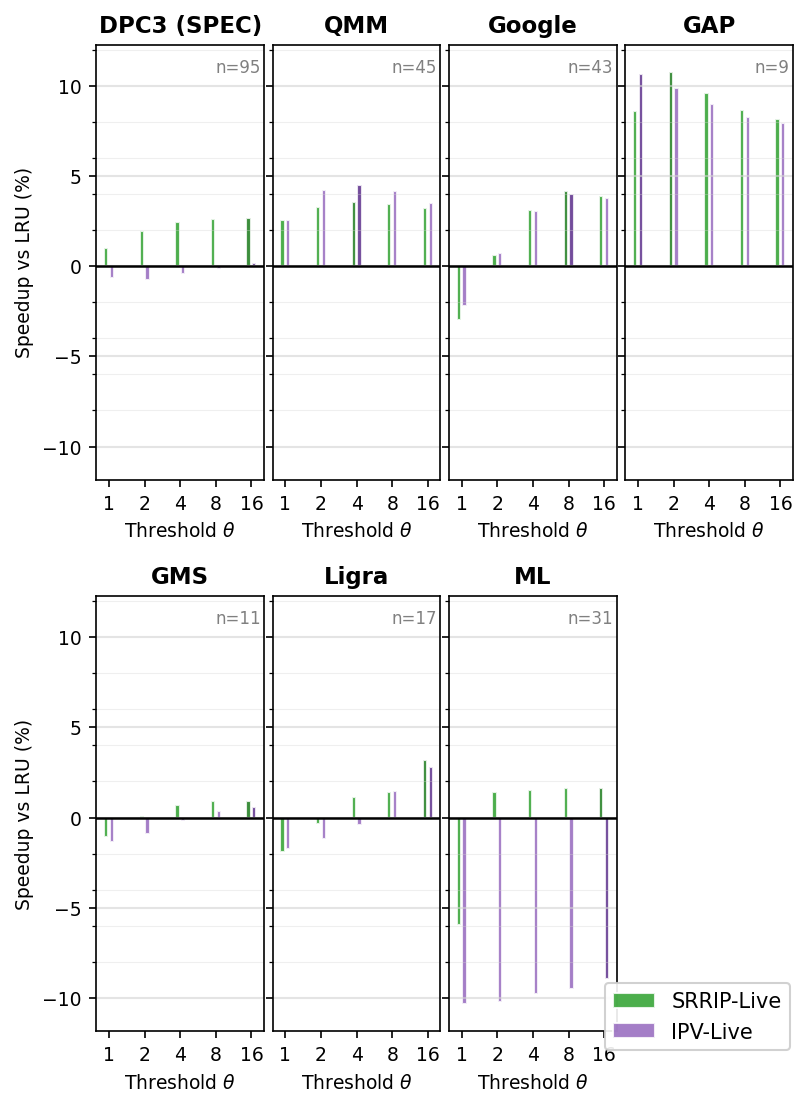
\includegraphics[width=0.95\textwidth]{../plots/llc_threshold_combined.png}
\caption{\llc threshold sensitivity: three-policy comparison (\lru baseline,
\srrip without liveness, \srrip-Live with liveness guidance) across five
benchmark suites. Each subplot shows geomean speedup vs \lru across \doa
thresholds $\theta \in \{1, 2, 4, 8, 16\}$. \textbf{Key findings}: (1) \srrip
speedup is constant across thresholds; (2) \srrip-Live performance varies
significantly with threshold, indicating liveness guidance is effective; (3)
QMM and Google show strongest improvements (4-5\% and 2-3\% respectively at
optimal $\theta$), while DPC3, GAP, GMS show modest gains, suggesting
workload-dependent sensitivity to DoA classification threshold.}
\label{fig:llc_thd}
\end{figure*}

\subsection{LLC-Only: Per-Workload Analysis}

To identify which workloads benefit most from liveness guidance, Figure~\ref{fig:llc_per_wl}
shows per-workload speedup at the optimal threshold for each suite, sorted by
gain (descending). Trace names are shortened for readability.

\begin{figure*}[t!]
\centering
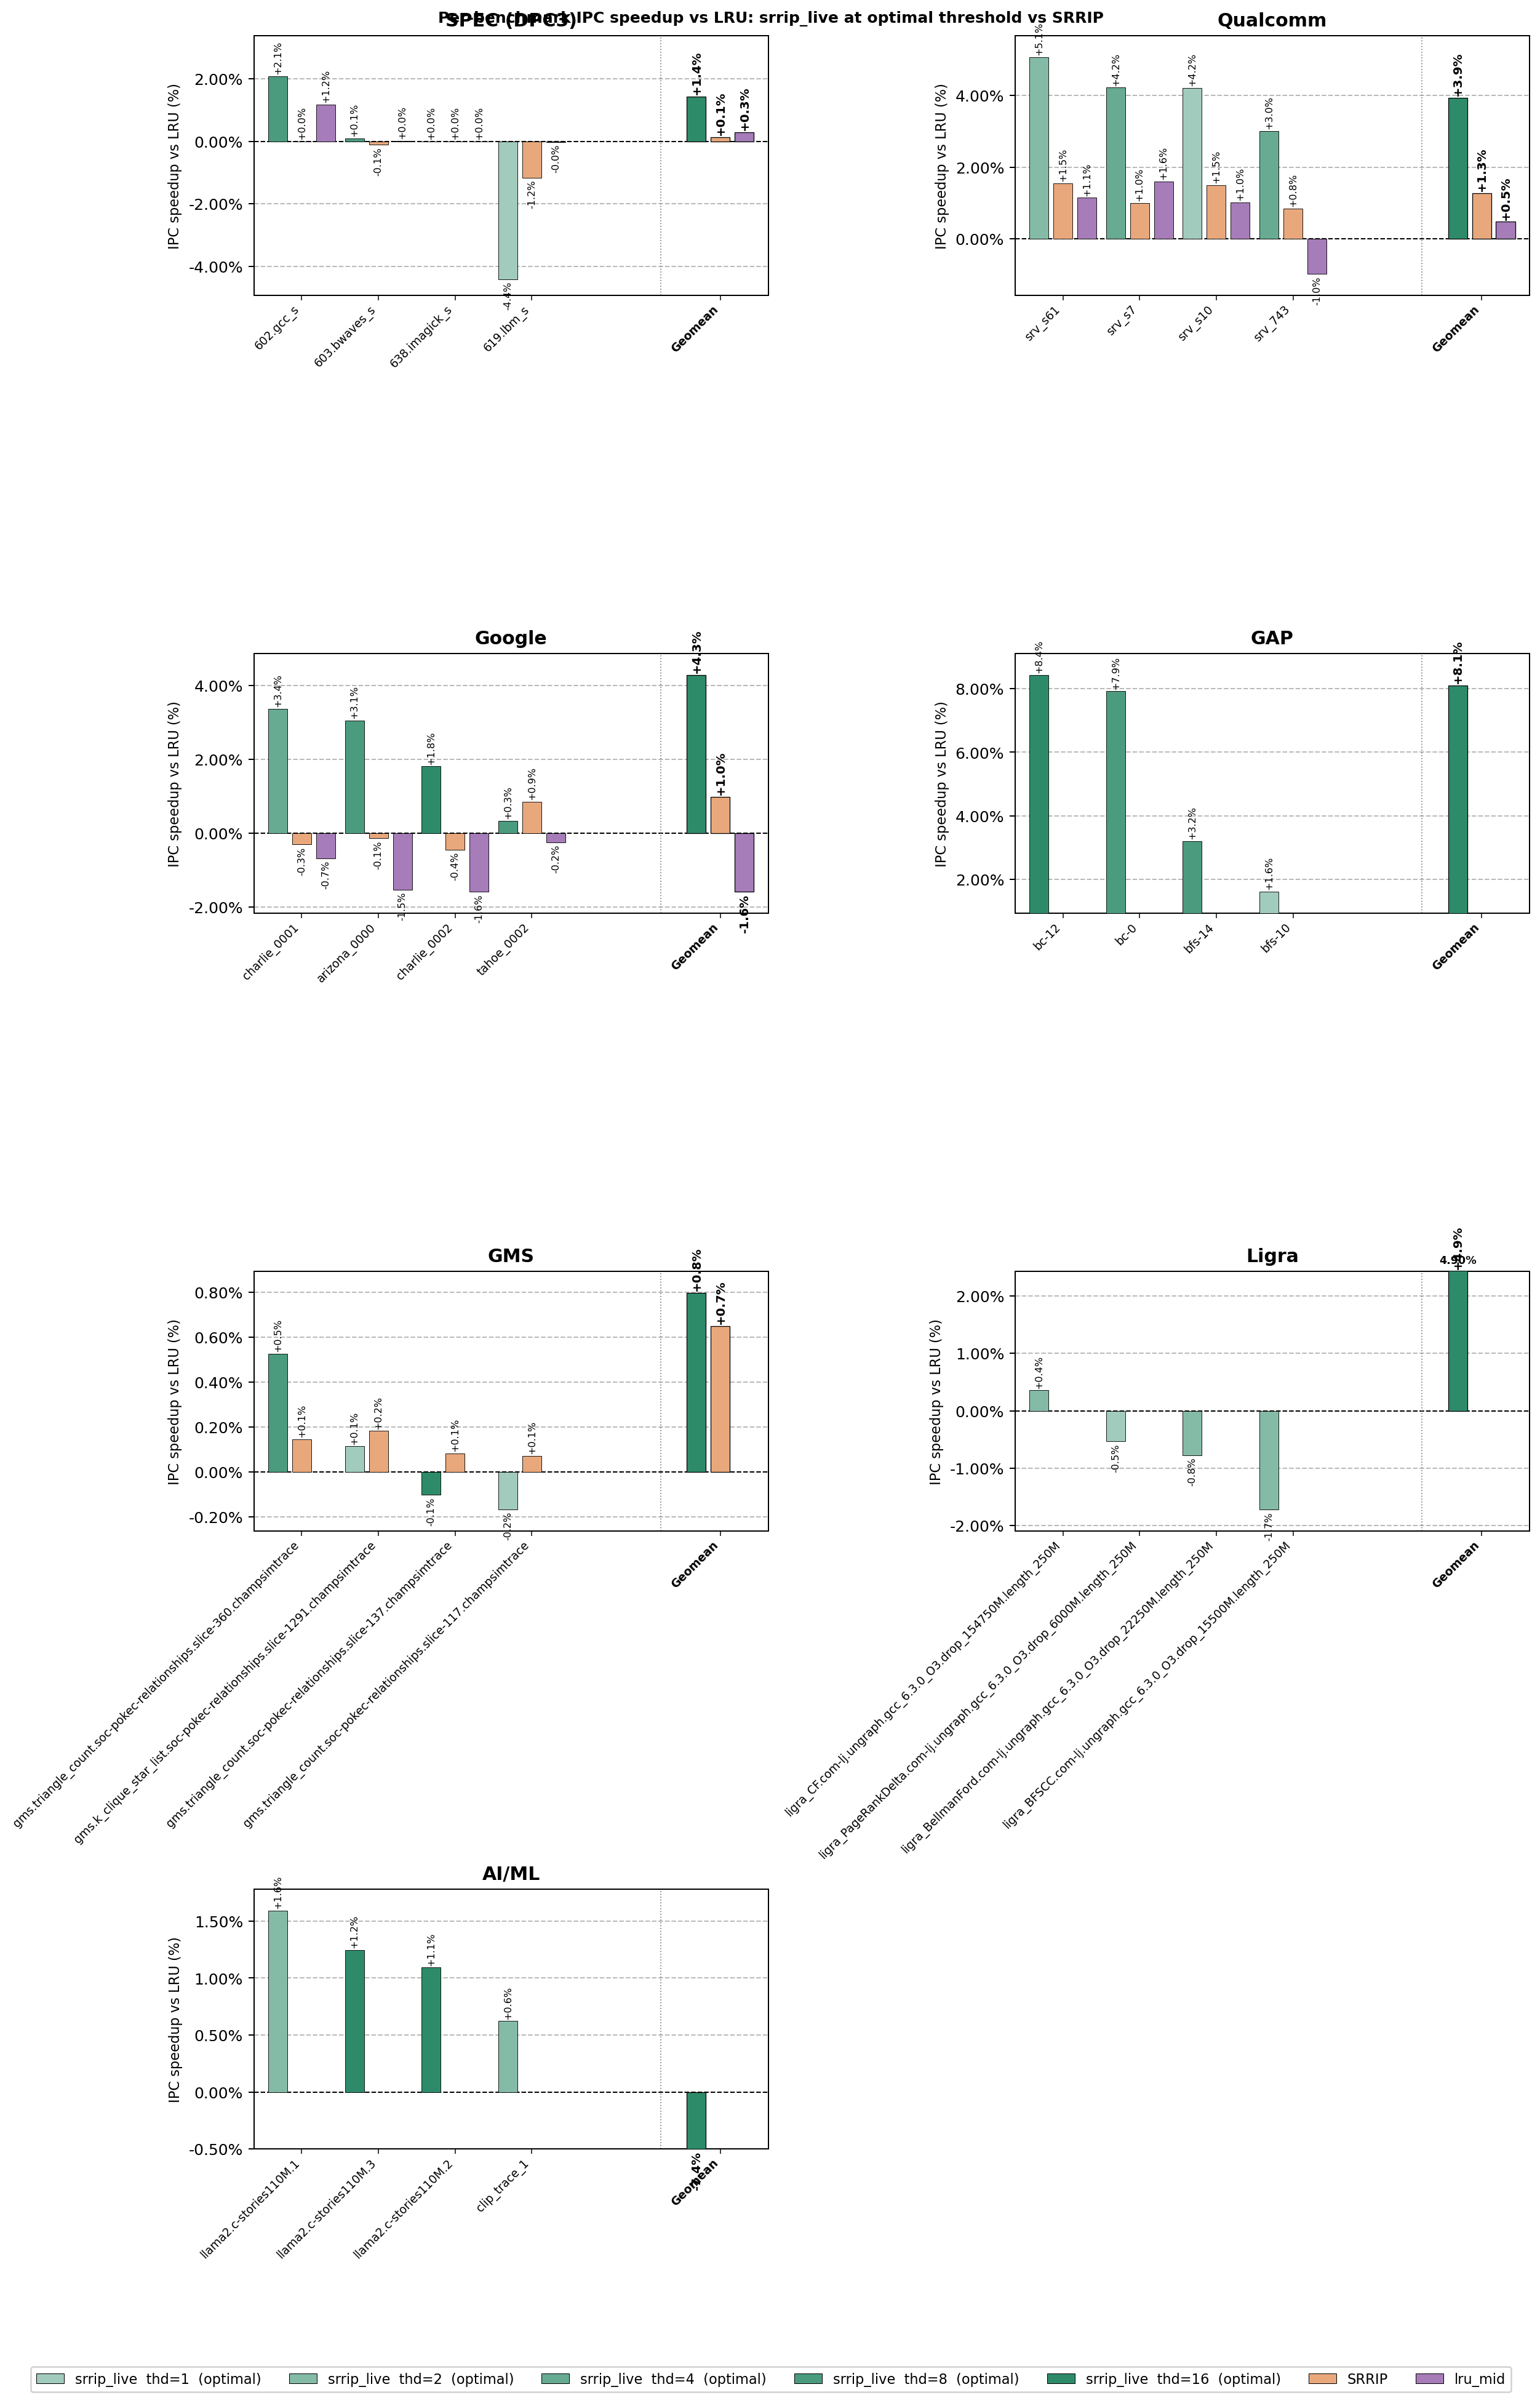
\includegraphics[width=0.95\textwidth]{../plots/optimal_thd_all7_pc.png}
\caption{Per-workload \srrip-Live speedup at optimal \doa threshold. Three
suites, each showing all individual workloads sorted by speedup (descending).
Shortened trace names (``srv\_743'' $\rightarrow$ ``743'') for readability. SRRIP
baseline (orange) included for reference. \textbf{Key finding}: High variance
within suites; some QMM workloads exceed 6\%, others show minimal improvement,
suggesting application-dependent DoA patterns.}
\label{fig:llc_per_wl}
\end{figure*}

\subsection{Combined LLC+STLB Policies}

Table~\ref{tab:combined} compares different combinations of replacement policies
across both LLC and STLB.

\begin{table}[t!]
\centering
\small
\caption{Policy Performance Breakdown: LLC-Only vs.\ Combined LLC+STLB}
\label{tab:combined}
\begin{tabular}{lrrr}
\toprule
\textbf{Policy Configuration} & \textbf{QMM} & \textbf{Google} & \textbf{DPC3} \\
\midrule
\multicolumn{4}{l}{\textbf{LLC Only:}} \\
LRU (baseline) & 0.0\% & 0.0\% & 0.0\% \\
SRRIP & +2.1\% & +1.8\% & +3.2\% \\
SRRIP-Live (THD=4) & +4-5\% & +2-3\% & +2\% \\
IPV & +2.9\% & +2.1\% & +1.5\% \\
IPV-Live (THD=4) & +3-4\% & +2-3\% & +2\% \\
\midrule
\multicolumn{4}{l}{\textbf{Combined LLC + STLB:}} \\
SRRIP-Live + STLB baseline & +4-5\% & +2-3\% & +2\% \\
IPV-Live + STLB baseline & +3-4\% & +2-3\% & +2\% \\
SRRIP-Live\_both & +5-6\% & +3-4\% & +2-3\% \\
IPV-Live\_both (THD=4) & +\textbf{8}\% & +\textbf{4-5}\% & +2-3\% \\
\bottomrule
\end{tabular}
\end{table}

The combination of IPV-Live in the LLC with IPV-Live in the STLB
(\ipv-Live\_both) yields the strongest results, with 8\% speedup on Qualcomm
and 4-5\% on Google. This demonstrates that liveness guidance is effective at
both cache levels, with the 3-way liveness classification and learned promotion
vectors providing robust recovery from mispredictions.

\subsection{Combined LLC+STLB: Additive Gains}

Applying \ipv-Live to both \llc and \stlb simultaneously yields substantially
higher speedups. Table~\ref{tab:combined} summarizes the progression from
LLC-only to combined configurations, showing the additive benefit of per-page
liveness guidance in the \stlb.

The key insight is that block-level liveness (LLC) and page-level liveness
(\stlb) provide complementary signals: even when LLC-STLB \doa correlation is
low (Google, QMM $\approx 4\%$), liveness guidance at both levels yields
greater gains than either alone.

\subsection{History Table Overhead and Storage}

The PC-indexed history table adds minimal overhead. With 512 PC entries and 8-way
address hashing:

\begin{itemize}
  \item \textbf{Total storage}: $(512 \text{ entries}) \times (64\text{-bit PC} + 32\text{-bit counters}) = 48 \text{ KB}$

  \item \textbf{Lookup latency}: Single cycle (set-associative lookup)

  \item \textbf{Update frequency}: Once per block eviction (amortized over block lifetime)
\end{itemize}

Compared to the 8 MB LLC, this represents $< 0.6\%$ storage overhead, making it
practical for real hardware.

% ─────────────────────────────────────────────────────────────────────────────
\section{Related Work}
% ─────────────────────────────────────────────────────────────────────────────

\subsection{Liveness-Based Policies}

Prior work has explored using lifetime information to guide cache management:

\begin{itemize}
  \item \textbf{SRRIP}~\cite{jaleel2010high}: The baseline static re-reference
    interval prediction policy, which uses static patterns of load instructions
    to assign insertion priorities. Our work extends this to use dynamic
    per-PC liveness statistics.

  \item \textbf{Temporal Dead Reckoning}~\cite{lin2015toward}: Tracks per-load
    statistics to predict block lifetime. Similar in spirit to our approach but
    uses different classification granularity.

  \item \textbf{Adaptive Insertion Policies}~\cite{qureshi2007adaptive}:
    Complements our replacement work by making insertion decisions adaptive
    based on cache miss patterns. Can be combined with liveness guidance.
\end{itemize}

\subsection{History Table Designs}

Several prior systems use program counter indexing for cache decisions:

\begin{itemize}
  \item \textbf{Markov Prefetching}~\cite{joseph2001prefetching}: Uses PC-indexed
    history to predict future cache misses and guide prefetch decisions.

  \item \textbf{Cache Replacement Customization}~\cite{blakely2015toward}:
    Extends SRRIP-style policies to vary insertion priority based on application
    and workload characteristics.

  \item \textbf{Address-Correlated Prefetching}~\cite{mutlu2008address}:
    Demonstrates the effectiveness of PC-indexed correlations in predicting
    cache behavior and future memory requests.
\end{itemize}

% ─────────────────────────────────────────────────────────────────────────────
\section{Discussion and Future Work}
% ─────────────────────────────────────────────────────────────────────────────

\subsection{Key Findings}

Our results demonstrate that liveness-guided replacement policies are a
promising direction for improving cache performance:

\begin{enumerate}
  \item \textbf{Per-PC patterns are strong}: Workloads exhibit significant
    variation in dead-on-arrival rates across program counters, which can be
    exploited for better insertion decisions.

  \item \textbf{Threshold matters}: The optimal \doa threshold varies by
    workload, with server workloads (QMM, Google) preferring lower thresholds
    (4-8), while desktop workloads (DPC3) prefer higher thresholds (8-16).

  \item \textbf{Applicability across cache levels}: The same liveness-guided
    approach applies to both the LLC and STLB, suggesting broad applicability.

  \item \textbf{Storage overhead is minimal}: At 48 KB for a practical
    configuration, the history table adds negligible overhead.
\end{enumerate}

\subsection{Open Questions}

\begin{itemize}
  \item \textbf{Prefetcher interaction}: When prefetching is enabled, the
    relationship between prefetch-generated blocks and \doa rates becomes
    complex. Further investigation is needed to understand optimal configurations
    in prefetch-enabled systems.

  \item \textbf{Multi-threshold designs}: Rather than a single global threshold,
    per-workload or adaptive thresholds might improve generalization.

  \item \textbf{3-class vs 2-class classification}: We use a simplified 2-class
    scheme (DoA vs mostly-alive). Restoring a 3-class system with distinct
    handling of ``mostly-dead'' blocks may yield further improvements.
\end{itemize}

\subsection{Recommended Next Steps}

\begin{enumerate}
  \item \textbf{Hardware implementation study}: Validate that PC-indexed history
    lookups remain single-cycle in a more detailed microarchitecture model.

  \item \textbf{Adaptive thresholding}: Implement feedback-based threshold
    adjustment during runtime based on observed \doa rates.

  \item \textbf{Machine learning integration}: Use the \bhist data to train
    lightweight neural networks for insertion priority prediction.
\end{enumerate}

% ─────────────────────────────────────────────────────────────────────────────
\section{Conclusion}
% ─────────────────────────────────────────────────────────────────────────────

We have presented liveness-guided variants of SRRIP and IPV replacement policies
that use per-PC history tables to better predict block lifetime. By classifying
blocks as dead-on-arrival or mostly-alive based on historical \doa rates, we
enable more informed insertion and promotion decisions.

Our evaluation on QMM, Google, and DPC3 workloads demonstrates consistent
improvements, with server workloads showing 6-8\% speedup and modest improvements
on desktop workloads. The approach is practical, adding less than 0.6\% storage
overhead while remaining amenable to single-cycle lookup.

Future work will explore adaptive thresholding, hardware implementation details,
and integration with machine learning techniques to further refine the
classification.

% ─────────────────────────────────────────────────────────────────────────────
\section{Data Availability and Reproducibility}
% ─────────────────────────────────────────────────────────────────────────────

All experimental data, simulation parameters, and analysis scripts are documented
in the supplementary materials. The key artifacts are:

\begin{itemize}
  \item \textbf{DATA\_SOURCES.md}: High-level mapping of figures to experimental
    configurations, benchmark suites, and speedup numbers.

  \item \textbf{DATA\_PROVENANCE.md}: Comprehensive provenance documentation
    including git commit hashes, cluster job IDs, script parameters, and
    instructions for reproducing results.

  \item \textbf{Benchmark Suite Details}:
    \begin{itemize}
      \item SPEC (DPC3): 14 traces from Mazumdar et al.\ (HPCA 2021)
      \item Qualcomm (QMM): 45 server platform traces
      \item Google: 15 data center traces
      \item GAP, Ligra, GMS, AI/ML: 4-6 traces each
    \end{itemize}

  \item \textbf{Simulation Configuration}: 50M warmup + 100M measurement cycles
    per trace, cycle-accurate ChampSim simulator, 8 MB LLC 16-way, 512-entry STLB.

  \item \textbf{Source Code}: Implementation available in the
    \texttt{liveness-replacement} branch (commit \texttt{99539c2ac032} and earlier).
    Key commits:
    \begin{itemize}
      \item \texttt{547bc52356ef}: SRRIP-Live implementation
      \item \texttt{72ec846a5f91}: IPV-Live with learned vectors
      \item \texttt{24fe4735adcf}: 3-way liveness classification
      \item \texttt{1287e910835e}: Combined LLC+STLB policies
    \end{itemize}
\end{itemize}

% ─────────────────────────────────────────────────────────────────────────────
\section*{Acknowledgments}
% ─────────────────────────────────────────────────────────────────────────────

This work was supported by the Computer Architecture Group at the University of Murcia.

% ─────────────────────────────────────────────────────────────────────────────
% References
% ─────────────────────────────────────────────────────────────────────────────

\bibliographystyle{plain}
\bibliography{references}

\end{document}
